\documentclass[11pt]{article}
\usepackage[letterpaper,margin=1in]{geometry}
\usepackage[T1]{fontenc}
\usepackage{lmodern,microtype,amsmath,amssymb,amsthm,booktabs,array,longtable,graphicx}
\usepackage{xcolor,enumitem}
\usepackage[section]{placeins}
\usepackage[colorlinks=true,linkcolor=blue!45!black,citecolor=blue!45!black,urlcolor=blue!45!black]{hyperref}
\usepackage{listings}
\lstset{basicstyle=\ttfamily\small,columns=fullflexible,breaklines=true,frame=single}
\newtheorem{proposition}{Proposition}
\newtheorem{lemma}{Lemma}
\newcommand{\dm}{\ensuremath{\Delta\text{-mean}}}
\newcommand{\meanw}{\overline{w}}
\newcommand{\meand}{\overline{d}}
\newcommand{\dist}{\operatorname{dist}}
\newcommand{\Var}{\operatorname{Var}}
\newcommand{\code}[1]{\texttt{#1}}
\setlength{\emergencystretch}{2em}
\setlist{nosep}
\newcommand{\GraphCount}{192}
\newcommand{\ValidationCount}{43,956}
\newcommand{\SelectionChanges}{21}
\newcommand{\SelectionCases}{48}
\newcommand{\AbstractFinding}{At $n=5000$, mean-width stepping has a sparse-graph speed ratio of 1.76 with append-only lists and 1.76 with duplicate suppression, relative to the author's standard-library-heap Dijkstra. The append-only solver reaches 1.97 at $n=10000$. Suppression changes the dense ratio at $n=5000$ from 0.06 to 0.56. A cyclic-container implementation gives 1.51--1.64 on the road inputs; the maximum-weight/maximum-degree rule is competitive. Degree-gated lookahead increases heap insertions in all 24 live core validation queries.}

\title{Bucket Width, Duplicate Work, and Local Lookahead\\in Sequential Shortest Paths}
\author{Bee Rosa Davis}
\date{September 2026}
\begin{document}
\maketitle
\begin{abstract}
Choosing a bucket width for $\Delta$-stepping is an implementation decision with
both algorithmic and measurement consequences. We study the mean-edge-weight
rule, degree-scaled alternatives, and a width selected on a separate source,
using a common sequential implementation. A factorial experiment separates
unchanged-label rescans from repeated heavy-edge processing. A second experiment
compares degree-gated one-hop relaxation with an identical never-scout baseline,
including exact admission and executed-work controls. The artifact contains
\GraphCount{} graph configurations, \ValidationCount{} validation timings, three
synthetic graph seeds, sparse graphs through $10^6$ vertices, and three DIMACS
road networks. Every measured solver is checked against reference distances.
\AbstractFinding{}
The study distinguishes a cheap useful default from a uniformly good rule, and
a selector that limits overhead from lookahead that improves the underlying
algorithm. GIGI supplies durable edge records and indexed incidence; its
normalized weight-variance statistic is assessed as a feature, with no metric
interpretation imposed on it.
\end{abstract}

\section{Questions and scope}
Single-source shortest paths on nonnegative weighted digraphs admit several
practical choices of work ordering. A heap exposes the smallest tentative
distance at each extraction; $\Delta$-stepping groups a range of distances and
revisits light-edge relaxations within that range~\cite{dijkstra,meyer}.
The relevant engineering question is which ordering pays for its bookkeeping
on a given input and machine.

We examine three questions. Does $\Delta=\meanw$, the mean stored arc weight,
offer a useful low-cost setting, with and without redundant bucket work? Does
degree-gated one-hop lookahead improve a heap solver, rather than merely reduce
the overhead of unrestricted lookahead? Can a graph database supply the
representation and features these decisions require without changing the graph
being solved?

The contribution is an experimentally delimited comparison with an inspectable
artifact: bucket-width rules share a solver, two sources are held out from
width calibration, mechanisms have removal controls, and storage semantics are
verified with planted distances. We establish elementary invariants needed to
interpret the experiments. We do not propose a new asymptotic SSSP bound or
extrapolate sequential timings to parallel implementations.

\paragraph{Related implementations.}
Rules that avoid a parameter search already exist. Parallel Boost documents
$w_{\max}/d_{\max}$ when the width is omitted~\cite{boost}. The historical
Gunrock v0.3 source estimates a width proportional to mean weight divided by
integer average degree, with a factor of 32 and an additional caller-supplied
multiplier~\cite{gunrock}. GAPBS exposes a fixed default of 1, while the inspected
Galois implementation exposes a bucket shift of 13 and warns about sensitivity
to that setting~\cite{gapbs,galois}. These are evidence of implemented defaults,
not interchangeable algorithms or claims about current GPU performance.
Dong et al. study parameter-sensitive parallel stepping algorithms~\cite{dong};
their measurements do not supply a universal error bar for this sequential study.
The present work makes no priority claim for a weight statistic.

\section{Model, rules, and representation}
Let $G=(V,E,w)$ be a finite directed multigraph, $n=|V|$, $m=|E|>0$,
$w:E\to\mathbb{R}_{\ge0}$, and $s\in V$. Parallel arcs are distinct records;
unreachable vertices have distance $+\infty$. The query computes a distance
vector for all vertices. It does not perform point-to-point early termination.
We use out-degree $d^+(v)$ and
\[
 \meanw=\frac1m\sum_{e\in E}w(e),\qquad
 \meand=\frac mn,\qquad
 w_{\max}=\max_e w(e),\quad d_{\max}=\max_v d^+(v).
\]
All graph statistics refer to the entire stored graph, including components
unreachable from $s$. The names \dm{}, GSR-1, GSR-$k$, and Hub-batch denote,
respectively, mean-width stepping, gated one-hop relaxation, its multi-hop
extension, and hub-oriented batching. Only \dm{} and GSR-1 are evaluated here;
the other names carry no measured performance claim in this study.

\paragraph{Width rules.}
The principal settings are $\meanw$, $\meanw/\meand$,
$\meanw/\sqrt{\meand}$, the median weight, the population standard deviation
$\sigma_w$, and $w_{\max}/d_{\max}$. Degree denominators in the implementation
are bounded below by 1. For median and standard deviation, a zero or tiny result
is floored at $10^{-6}\meanw$. All measured instances have positive mean weight;
an all-zero graph is separately tested with width 1. The degree-scaled rules
are dimensionally compatible heuristics. Their use here is not an application
of a random-graph complexity theorem outside its hypotheses.

\paragraph{Stored layout.}
An adjacency list stores each arc as a destination index and a binary64 weight.
The default ordering is ascending weight; explicit layout experiments change
that ordering. Vertices have an independent registry, so a vertex with no
incident arcs remains part of the output. Minimum-weight parallel-arc reduction
would preserve shortest distances but change $m$, $\meanw$, the admission rate,
and operation counts. We therefore retain the input arcs.

\begin{proposition}[Global scaling and irrelevant components]
In exact arithmetic, multiplying every arc weight and the bucket width by the
same $a>0$ preserves bucket indices and all strict relaxation comparisons.
Nevertheless, $\meanw$ is not a source-local statistic: adding an unreachable
component can change it by an arbitrarily large factor without changing any
distance from $s$ to the original vertices.
\end{proposition}
\begin{proof}
Every finite tentative distance scales by $a$, and
$\lfloor ad/(a\Delta)\rfloor=\lfloor d/\Delta\rfloor$. For the second claim,
add an isolated directed arc of weight $M$ between two new vertices. The mean
becomes $(m\meanw+M)/(m+1)$ while all original source paths are unchanged.
\end{proof}
This observation limits what any global-width statistic can encode. The artifact
tests the disconnected-component construction and a power-of-two rescaling;
the latter avoids introducing an extra rounding perturbation in binary64.

\section{Algorithms and mechanism controls}
\subsection{Bucket closure with duplicate suppression}
For $\Delta>0$, bucket $i$ represents $[i\Delta,(i+1)\Delta)$. Arcs of weight at
most $\Delta$ are light. Let $D[v]$ be the current label and $L[v]$ the label at
which the outgoing light arcs of $v$ were last scanned. Both begin at infinity,
except $D[s]=0$. A successful relaxation appends a vertex identifier to the
bucket of its new label. Entries may become stale; they are not deleted eagerly.

\begin{center}
\begin{minipage}{0.94\linewidth}
\begin{lstlisting}[mathescape=true]
while some bucket is nonempty:
    i = smallest nonempty bucket index; R = empty vertex set
    while bucket i is nonempty:
        remove its current list of entries
        for each entry u:
            skip unless floor(D[u] / Delta) == i
            skip if D[u] == L[u]
            L[u] = D[u]; add u to R
            relax every light outgoing arc of u
    for each u in R, once:
        relax every heavy outgoing arc using the final D[u]
\end{lstlisting}
\end{minipage}
\end{center}

\begin{lemma}[Safe suppression]
Skipping a repeated light scan at an unchanged label preserves all labels
attainable by relaxation. Once light closure is reached in bucket $i$, scanning
each heavy outgoing arc of a vertex in $R$ once at its final label suffices.
\end{lemma}
\begin{proof}
An unchanged source label offers the same candidate value on each outgoing arc;
destination labels only decrease. No candidate rejected on an earlier identical
scan can become a strict improvement later. If the source label decreases,
the equality test fails and the light scan is allowed. At closure, the final
label of a vertex is no greater than any earlier label used in that phase.
Its final heavy-arc candidate dominates all earlier candidates on that arc.
A heavy arc cannot return a label to bucket $i$, because its weight exceeds
$\Delta$. Thus delayed heavy processing does not reopen the closed bucket.
\end{proof}
The smallest-bucket invariant is that, when phase $i$ begins, every vertex whose
shortest distance is below $i\Delta$ has its exact label and has propagated its
outgoing relaxations. Nonnegative weights and light closure then finalize the
vertices of the current interval before advancing. Together with this invariant,
safe suppression gives the same
shortest distances as $\Delta$-stepping~\cite{meyer}. The implementation maintains
one generation mark per vertex for membership in $R$. No sorting or hashing of
the touched vertices is required.
The exact comparison $D[u]=L[u]$ compares a stored label with its saved copy;
it does not recompute a path sum. A strict decrease therefore permits another scan.

The factorial control changes two switches independently: suppress unchanged
light scans; deduplicate heavy work. The list/list arm retains every heavy-arc
copy produced by every light scan. The skip-only and heavy-only arms isolate the
two costs. All four use the same width, relaxation order within a scan, and map
container. All four execute the same bookkeeping code; the switches determine
whether its suppression effects apply. List is the author's append-only
mean-width solver, retained unchanged as an additional comparison; it also
computes $\meanw$ inside each solve.

\paragraph{Containers and accounting.}
We compare an ordered map of bucket lists with a cyclic array. The array has
$\lceil w_{\max}/\Delta\rceil+2$ slots, each tagged with its absolute bucket
index. During a phase, successful new labels lie at most $w_{\max}$ above a
label in the current interval; this bounds the simultaneously relevant bucket
indices. Generation tags detect aliasing. The cyclic cursor may inspect empty
indices, whereas the map jumps to its smallest occupied key. Consequently a
small live window is a space property, not a proof that either container wins.
The ratio $w_{\max}/\Delta$ is measured rather than assumed constant.

Deduplicated heavy relaxations visit each reachable vertex's heavy arcs at most
once after its bucket closes. Light scans can repeat after genuine improvements.
Our implementation scans adjacency lists to classify arcs and again to select
heavy arcs, so adjacency inspections and heavy relaxations are distinct counters.
It does not claim to be an optimized CSR or parallel implementation.

\subsection{Gated one-hop relaxation}
GSR-1 uses lazy heap deletion and ordinary settled flags. When settling $u$
improves $D[v]$, it may immediately scan the outgoing arcs of the unsettled
vertex $v$, before inserting $v$ into the heap. These speculative relaxations
do not settle $v$. The fixed gate admits $(u,v)$ precisely when
$d^+(u)\le4$ and $d^+(v)\le4$.

\begin{proposition}[Degree normalization]
For $\meand>0$, $\kappa(v)=(d^+(v)-\meand)/\meand$ is an affine function of
out-degree. A threshold on $\kappa$ supplies exactly the same ordering of
vertices as a threshold on degree.
\end{proposition}
\begin{proof}
$\kappa(v)=d^+(v)/\meand-1$ has positive slope $1/\meand$.
\end{proof}
We call this quantity normalized degree deviation. No curvature assumption is
needed for the gate or its correctness. Every speculative improvement represents
an actual source walk and is queued. Ordinary minimum-label extraction therefore
retains the Dijkstra invariant; extra relaxations may change work, not distances.

The necessary baseline is \emph{NEVER}, implemented by the same heap path with
no scouting. \emph{ALWAYS} measures unrestricted scouting. \emph{HIGH/HIGH}
uses $d^+(u)>4\land d^+(v)>4$; the logical complement instead uses $\lor$.
Tail-only, head-only, and $\tau=\max(3,\lfloor\meand/2\rfloor)$ gates complete
the deterministic controls. A gate is live, saturated, or dead when it admits
some, all, or no graph arcs. Only live cases can distinguish selection from the
two extremes.

Five seeded random masks admit exactly the same number of graph arcs as the
degree gate. This does not equalize executed scouts: a scout requires a successful
relaxation and an unsettled head. Nor does it equalize work: scanning $v$ costs
$d^+(v)$ arc inspections. Additional random-mask arms cap executed scout-arc
work at the degree gate's measured amount on that query. A whole scout must fit
the remaining budget, so the cap can be underspent. We report both admission and
execution rather than infer one from the other.

\subsection{Heap, integer, and certified-relaxation baselines}
The timing reference, labeled Std heap, is the author's Dijkstra implementation
using Rust's standard-library binary heap, lazy deletion, and settled flags.
No externally maintained SSSP solver is timed. A shared explicit
heap implementation supplies binary and 4-ary variants and counts comparisons,
pushes, pops, stale pops, and maximum occupancy. Integer inputs additionally use
a monotone radix heap~\cite{radix}. Floating inputs are never rounded to create
an integer competitor. The radix implementation uses lazy duplicates; we do not
ascribe the decrease-key complexity bound of a different implementation to it.

The caliber control uses the minimum incoming weight
$c(v)=\min_{(u,v)\in E}w(u,v)$~\cite{goldberg}. At the start of a heap-extraction
phase, let $\mu$ be its valid minimum label. A newly improved vertex with
$D[v]\le\mu+c(v)$ may be placed on a free-processing stack instead of receiving
a new heap entry. The value $\mu$ is held fixed while that stack drains.
Previously queued entries for a subsequently settled vertex remain stale.

\begin{lemma}[Certificate used by the caliber control]
If $\mu$ is a lower bound on the exact distances of all vertices unsettled at
the start of a phase, a tentative label $D[v]\le\mu+c(v)$ is exact.
\end{lemma}
\begin{proof}
Any improvement not already propagated from the settled region must enter $v$
from a vertex whose distance is at least $\mu$, through an arc of weight at
least $c(v)$. Its length is at least $\mu+c(v)$. A tentative label is the length
of an actual walk, so it cannot lie below the shortest distance. Equality is
safe because relaxations require strict improvement.
\end{proof}
This control tests a certificate that can avoid a queue insertion. GSR-1 merely
moves relaxations earlier. The two mechanisms should not be conflated.

\section{Experimental design}
\subsection{Instances and machine}
\begin{table}[tb]\centering\small\setlength{\tabcolsep}{3.5pt}
\caption{Completed primary panels. Configurations include paired transformations of the same topology, so they are not all independent graph draws. Sources shown are for validation; calibration uses source 0.}
\begin{tabular}{lrrrr}
\toprule
Panel & Configs. & Seeds & Sources & Rounds \\ \midrule
Core synthetic & 54 & 3 & 2 & 12 \\
Density & 48 & 3 & 2 & 8 \\
Weight laws & 48 & 3 & 2 & 8 \\
Sparse scale & 9 & 3 & 2 & 6 \\
DIMACS roads & 3 & -- & 6 & 8 \\
Layout & 30 & 3 & 2 & 8 \\
\bottomrule\end{tabular}\end{table}

The synthetic seeds are 42, 1729, and 2026. Sparse graphs draw an out-degree
uniformly from $\{1,\ldots,8\}$ and distinct nonself destinations, with weights
uniform on $[1,100)$. The core generator shuffles all possible destinations;
the scale panel samples destinations by rejection. These induce the same stated
distribution but do not produce identical seeded instances. We label the latter
\code{sparse\_fast} and record an arc/weight fingerprint for every configuration.

Dense graphs include each ordered nonself pair independently with probability
0.1. The density panel varies expected out-degree from 2 to 256 at $n=1000$
and 5000. Grids use the largest divisor of $n$ not exceeding $\sqrt n$ as their
row count; thus their reported size is exact. Adjacent grid vertices have two
opposite arcs with the same weight in $[1,10)$.

Clustered graphs have clusters of size 50, internal directed inclusion probability
0.5 with weights in $[1,10)$, and two links per cluster pair in each direction
with weights in $[50,100)$. The complete cluster-level connectivity makes expected
degree grow with the number of clusters. This is not a fixed-degree scaling
experiment. Road-like synthetic graphs connect each point in the unit square to
its six nearest neighbors, with weight $\max(0.001,100rU)$, where $r$ is Euclidean
distance and $U$ is uniform on $[0.8,1.2)$. Only this generator uses coordinates.

The DIMACS distance graphs NY, BAY, and COL contain 264,346/733,846,
321,270/800,172, and 435,666/1,057,066 vertices/arcs, respectively.
They are downloaded without arc modification from the challenge collection,
whose maintainers disclose map-data defects~\cite{dimacs}. Compressed and
uncompressed SHA-256 digests are included in the artifact.

Runs use one software thread on an Intel Core i7-13620H, 64 GB RAM, Windows 11,
and Rust 1.92.0 targeting \code{x86\_64-pc-windows-msvc}; release settings are
optimization level 3, LTO, and one code-generation unit. Processor affinity and
priority remain at operating-system defaults. Campaign processes run sequentially,
without concurrent compilation or rendering by the experimenter. Frequency,
thermal state, core migration, and unrelated OS activity are uncontrolled.
Windows' \code{Win32\_Processor.L3CacheSize} reports 24,576 KiB (24 MiB),
recorded in the artifact. At one million vertices, arc payload alone
is about 72 MB; even dense $n=5000$ has about 40 MB of arc payload. Vertex count
alone cannot justify an in-cache claim.

\subsection{Correctness and timing}
Before timing each graph/source/arm, the harness checks its complete distance
vector against the standard-library-heap Dijkstra reference, both with and without instrumentation.
Finite distances allow relative error $10^{-10}$ with an absolute floor of
$10^{-10}$; unreachable status must agree exactly. This is a numerical agreement
test, not a claim of bitwise identity. Small seeded graphs are independently
checked by Bellman--Ford across all four duplicate-control settings. Separate
zero-cycle, parallel-arc, and isolate fixtures use the standard-heap solver or
explicit planted distances as their check. The integer path-length bound
is below $2^{53}$ on the radix inputs.

Validation uses 12 rounds per arm in the core panel, eight in density, laws,
roads, and layout, and six at scale. Adjacent rounds use one seeded random
permutation of the arms and its reverse, balancing position. Checks also warm
the code and graph. Returned vectors pass through \code{black\_box}. Internal
queue cleanup is timed; destruction of the returned vector is outside the timer.
Graph construction/loading, feature extraction, and width preparation are recorded
separately. Counter increments compile out of the timed instantiation.

Source 0 calibrates a map-based deduplicated solver over
\[
 \Delta/\meanw\in\{0.03125,0.05,0.1,0.25,0.5,0.75,1,1.5,2,4,8,16\}.
\]
Each candidate receives six balanced rounds. The smallest training median selects
one width; it is then timed alongside the named rules on held-out sources
$\lfloor n/3\rfloor,\lfloor2n/3\rfloor$. Road validation uses six sources
$\lfloor jn/7\rfloor$, $1\le j\le6$. We call this a \emph{selected grid width}.
It is neither a continuous optimum nor the fastest width on every source. The
grid contains 1 exactly, so a mean rule winning during validation cannot be
explained by the grid omitting that candidate.
The minimizing multiplier and its \code{selected\_grid} rows are session-specific:
a fresh laws-panel run selects a different multiplier on \SelectionChanges{} of
\SelectionCases{} configurations.

Each raw row retains the configuration, seed, source, arm, round, order position,
duration, width, and preparation cost. Per-query summaries include the median
and IQR of the \emph{paired time differences}, not just the baseline IQR. A
geometric ratio averages log paired ratios within seed and then across seeds.
The displayed bootstrap bands resample the three graph seeds, keeping sources
together. With only three seeds these bands are descriptive; they are not strong
population guarantees or an equivalence test. DIMACS sources belong to one graph
per region and do not become independent graph replicates.

\section{Results}
\subsection{Width choice after controlling implementation work}
\begin{table}[tb]\centering\small\setlength{\tabcolsep}{3.5pt}
\caption{Median solve time in milliseconds, taking the median of query medians across three seeds and two held-out sources. List is the author's append-only mean-width solver, retained unchanged; Map and Ring use both duplicate controls. Selected uses a width calibrated on source 0. Preparation is excluded except for the mean computation inside List.}
\begin{tabular}{lrrrrrrrr}
\toprule
Family & $n$ & Std heap & 4-ary & List & Map & Ring & $\meanw/\meand$ & Selected \\ \midrule
Sparse & 1,000 & 0.178 & 0.193 & 0.123 & 0.129 & 0.119 & 0.155 & 0.116 \\
Sparse & 2,000 & 0.394 & 0.415 & 0.229 & 0.238 & 0.226 & 0.298 & 0.231 \\
Sparse & 5,000 & 1.047 & 1.103 & 0.543 & 0.592 & 0.571 & 0.698 & 0.572 \\
Sparse & 10,000 & 2.378 & 2.498 & 1.214 & 1.339 & 1.277 & 1.429 & 1.180 \\
Clustered & 1,000 & 0.344 & 0.324 & 0.327 & 0.275 & 0.255 & 0.425 & 0.247 \\
Clustered & 2,000 & 0.822 & 0.791 & 0.615 & 0.535 & 0.514 & 0.832 & 0.526 \\
Clustered & 5,000 & 2.691 & 2.639 & 1.800 & 1.511 & 1.395 & 1.970 & 1.422 \\
Clustered & 10,000 & 7.259 & 7.436 & 6.699 & 3.981 & 3.891 & 4.742 & 3.948 \\
Dense & 1,000 & 0.772 & 0.668 & 4.821 & 0.849 & 0.873 & 0.862 & 0.637 \\
Dense & 2,000 & 2.378 & 2.014 & 22.875 & 3.193 & 3.306 & 2.931 & 2.562 \\
Dense & 5,000 & 9.303 & 7.982 & 146.659 & 16.625 & 16.991 & 13.857 & 13.520 \\
Grid & 1,000 & 0.101 & 0.111 & 0.101 & 0.103 & 0.102 & 0.124 & -- \\
Grid & 2,000 & 0.213 & 0.224 & 0.174 & 0.192 & 0.187 & 0.232 & -- \\
Grid & 5,000 & 0.563 & 0.607 & 0.415 & 0.475 & 0.444 & 0.546 & -- \\
Grid & 10,000 & 1.189 & 1.285 & 0.773 & 0.872 & 0.814 & 0.983 & -- \\
Roadlike & 1,000 & 0.108 & 0.118 & 0.127 & 0.126 & 0.125 & 0.148 & -- \\
Roadlike & 2,000 & 0.218 & 0.241 & 0.218 & 0.230 & 0.224 & 0.274 & -- \\
Roadlike & 5,000 & 0.582 & 0.617 & 0.507 & 0.545 & 0.524 & 0.641 & -- \\
\bottomrule\end{tabular}\end{table}

On sparse graphs, the seed-aggregated mean/map speed ratios are 1.43, 1.63, 1.76, 1.81 at $n=1000,2000,5000,10000$, respectively. The corresponding ratios of the list implementation are 1.42, 1.66, 1.76, 1.97. These are a measured sequence, not an asserted monotone scaling law. On clustered graphs at $n=5000$, the mean/map ratio is 1.84; the 4-ary heap ratio is 1.02. On dense graphs at that size, the list and mean/map ratios are 0.063 and 0.564. Removing duplicate work changes the magnitude of the slowdown; its residual must still be measured.
For sparse at $n=5000$, the descriptive seed interval for that ratio is [1.69, 1.81]. As a within-query example, seed 42, source 1666 has paired median margin 0.505 ms with middle-half interval [0.424, 0.547] ms. For clustered at $n=5000$, the descriptive seed interval for that ratio is [1.81, 1.88]. As a within-query example, seed 42, source 1666 has paired median margin 1.294 ms with middle-half interval [1.012, 1.370] ms. 
Across the List, Map, and Ring mean-width implementations, grid ratios range from 0.95 to 1.56. Across the List, Map, and Ring mean-width implementations, roadlike ratios range from 0.86 to 1.13. The road-network gains below refer to DIMACS inputs, not the six-neighbor synthetic generator. List reaches its largest reported sparse ratio at $n=10000$; Ring has larger ratios at the three smaller sparse sizes.

\begin{figure}[tb]
\centering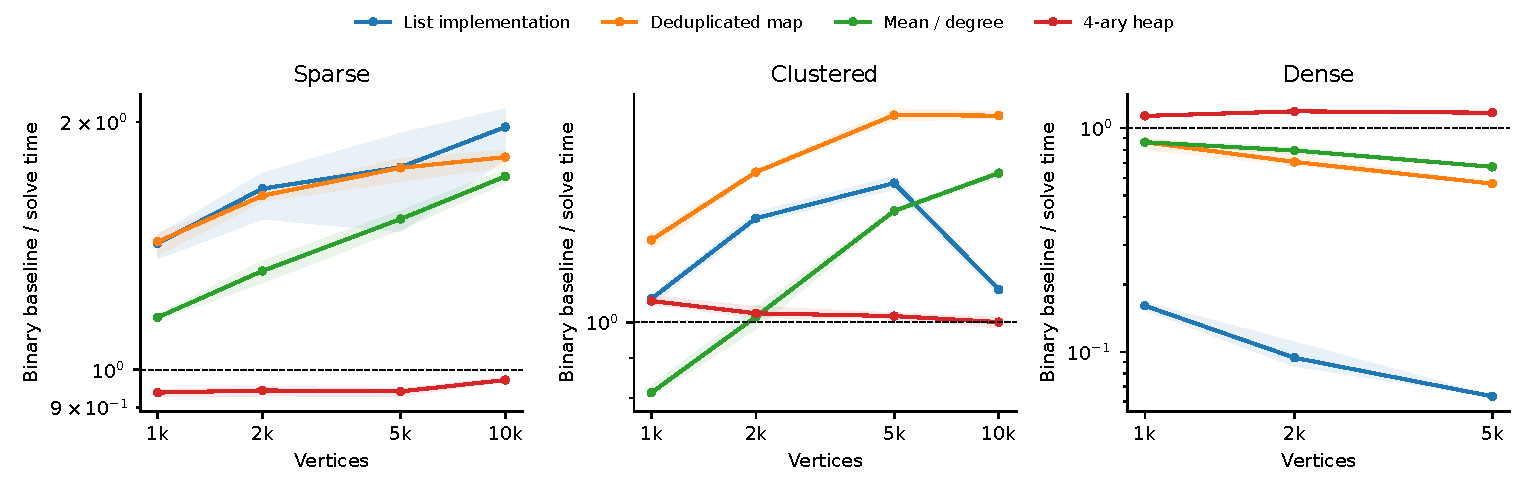
\includegraphics[width=\linewidth]{figs_v3/core.pdf}
\caption{Sequential solve-time ratios against the standard-library binary heap. Above 1
favors the plotted arm. Bands are descriptive graph-seed bootstrap intervals.
Each panel compares arms within the same validation rounds.}
\label{fig:core}
\end{figure}
\begin{table}[tb]\centering\small\setlength{\tabcolsep}{3.5pt}
\caption{Median operation counts at $n=5000$, same mean width and map container. Vertex scans omit skipped entries; heavy relaxations count evaluated heavy candidates.}
\begin{tabular}{llrrr}
\toprule
Family & Controls & Vertex scans & Heavy relaxations & Phases \\ \midrule
Sparse & List/list & 5,848 & 13,133 & 8 \\
Sparse & Skip only & 5,094 & 11,404 & 8 \\
Sparse & Heavy only & 5,848 & 11,063 & 8 \\
Sparse & Both & 5,094 & 11,063 & 8 \\
Clustered & List/list & 10,418 & 41,098 & 11 \\
Clustered & Skip only & 5,556 & 21,978 & 11 \\
Clustered & Heavy only & 10,418 & 19,800 & 11 \\
Clustered & Both & 5,556 & 19,800 & 11 \\
Dense & List/list & 29,540 & 7,383,816 & 2 \\
Dense & Skip only & 8,271 & 2,065,778 & 2 \\
Dense & Heavy only & 29,540 & 1,249,712 & 2 \\
Dense & Both & 8,271 & 1,249,712 & 2 \\
\bottomrule\end{tabular}\end{table}

\par\begin{samepage}
The planted mechanism fixture has arcs $(0,1,1)$, $(0,2,2)$, $(0,3,9)$,
$(1,3,2)$, $(2,3,3)$, and $(3,4,100)$ at $\Delta=10$. Vertex 3 acquires both
an obsolete and an improved entry in the same bucket. The list/list arm scans
one unchanged label and retains two copies of the heavy arc; enabling both
controls leaves one heavy relaxation and fewer vertex scans. Removing the
$(0,3,9)$ arc preserves distances but removes that redundancy. This fixture makes
the work claim falsifiable independently of timing.\par
\end{samepage}

\subsection{Density and weight distribution}
\begin{figure}[tb]
\centering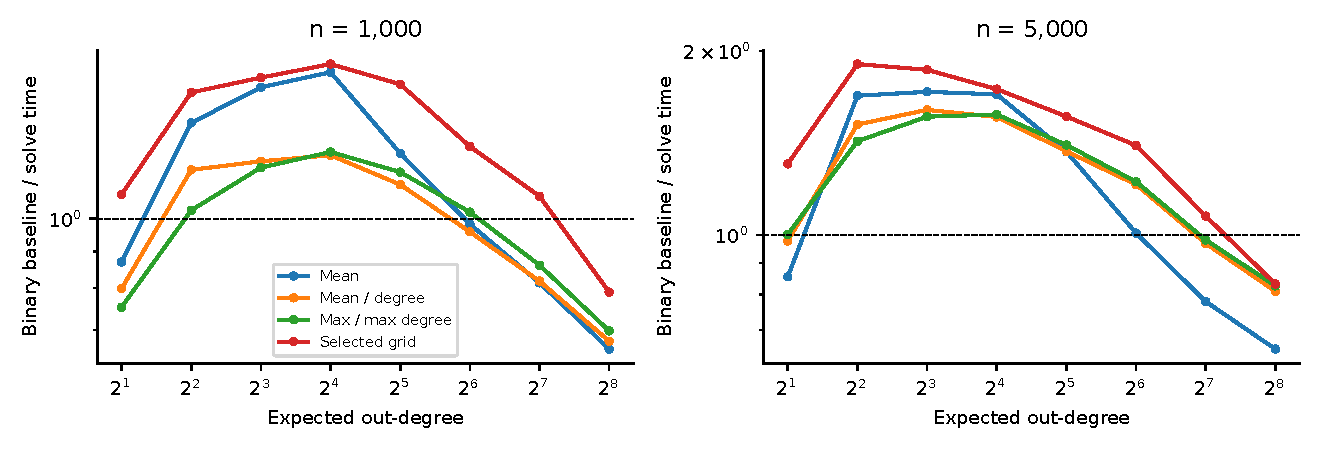
\includegraphics[width=.94\linewidth]{figs_v3/density.pdf}
\caption{Degree sweep on directed independent-edge graphs. The mean-degree
correction and maximum-degree rule are distinct settings. The selected grid
width is trained on source 0 and validated on different sources.}
\label{fig:density}
\end{figure}
At $n=5000$, the mean/map ratios span 0.65--1.71 across the degree sweep, while mean/degree/map spans 0.81--1.60. The mean/map ratio is 0.85 at expected degree 2, with a descriptive seed interval spanning 1, and 1.01 at degree 64. At expected degree 256 the two ratios are 0.65 and 0.81. Figure~\ref{fig:density} shows the full transition rather than identifying a universal cutoff from one dense endpoint.

When all weights are at least 1 and $\meanw/\meand<1$, the corrected rule has
no light arcs. A gain in that regime cannot be attributed to light-edge closure;
it is a different bucket schedule. Mean degree is therefore not a complete
description of the mechanism. The probability mass below the chosen width and
the distribution of tentative-label improvements also matter.

The law panel holds topology fixed while applying near-constant, skewed,
bimodal, zero-containing, and integer laws, a permutation of the weight multiset,
and multiplication by 1024. The permutation changes weight placement without
changing any global weight statistic. Across these law/topology combinations, the mean/map ratio ranges from 1.00 (clustered\_bimodal) to 1.92 (sparse\_bimodal). The full paired margins and named-rule timings are retained in the artifact.

These controls rule out interpreting a result on independent uniform weights as
a universal statement about geometric structure or about all nonnegative inputs.

\subsection{Larger graphs, real roads, and layout}
\begin{table}[tb]\centering\scriptsize\setlength{\tabcolsep}{2.5pt}
\caption{Median solve milliseconds at scale and on DIMACS roads. Scale has three seeds and two sources; each road graph has six sources. Max/degree uses the Boost-documented width in our map solver; Selected calibrates that solver on source 0. Radix uses unchanged integer weights.}
\begin{tabular}{lrrrrrrrrrr}
\toprule
Input & $n$ & Std heap & 4-ary & Map & Ring & $\meanw/\meand$ & Max/degree & Selected & Caliber & Radix \\ \midrule
sparse\_fast & 10,000 & 2.85 & 2.96 & 1.81 & 1.62 & 1.73 & 1.81 & -- & 2.62 & -- \\
sparse\_fast & 100,000 & 50.67 & 51.15 & 28.41 & 27.62 & 27.29 & 27.39 & -- & 45.90 & -- \\
sparse\_fast & 1,000,000 & 796.94 & 801.00 & 449.36 & 445.24 & 450.58 & 447.29 & -- & 779.67 & -- \\
NY & 264,346 & 51.62 & 54.71 & 34.14 & 31.29 & 35.87 & 29.68 & 29.72 & 42.61 & 66.92 \\
BAY & 321,270 & 54.79 & 59.67 & 41.31 & 36.51 & 43.95 & 35.45 & 35.02 & 43.64 & 78.50 \\
COL & 435,666 & 77.75 & 79.45 & 55.99 & 48.91 & 62.26 & 50.52 & 49.12 & 60.83 & 107.24 \\
\bottomrule\end{tabular}\end{table}

At one million vertices, mean/map and mean/ring have ratios 1.81 and 1.82 against the binary reference; the 4-ary ratio is 1.01. On NY, BAY, and COL, respectively, the mean/ring ratios are 1.64, 1.51, 1.57; the radix ratios are 0.76, 0.71, 0.72. These integer-road comparisons are necessary context for any advantage over one binary-heap implementation.
The maximum-weight/maximum-degree ratios on NY, BAY, and COL are 1.74, 1.57, 1.55, and the selected-width ratios are 1.73, 1.58, 1.57. The largest within-road spread among these two search-free implementations and calibration is 5.7\%. This comparison includes a container difference: the mean rule uses Ring here, whereas the other two use Map. It does not establish a resolved winner for small differences.

The scale generator and the road inputs extend the working set substantially,
but represent different distributions. Ratios across these panels are not a
scaling curve for one graph family. The layout panel preserves arcs and weights,
and remaps each source under vertex relabeling. Degree-sorted breadth traversal
and its reverse supply BFS/RCM-style orderings; the root policy is least degree
within an unvisited component. The implementation does not perform a separate
pseudo-peripheral-root search. All corresponding distances are checked after
mapping back. For $n=100000$, median ring solve times are 24.353 ms in weight order, 29.913 ms in destination order, 29.317 ms in random adjacency order, 25.681 ms after BFS relabeling, and 27.329 ms after reversal. Layout preparation is recorded separately; these figures describe solve time only.
The layout summary excludes both sources of case 29 (BFS, $n=100000$, seed 2026), flagged during review for background synchronization interference. BFS at that size consequently has two seeds and four queries; other layouts retain three seeds and six queries. Raw samples, including the excluded case, remain available.


\subsection{Gates and the cost of speculative work}
\begin{table}[tb]\centering\small\setlength{\tabcolsep}{3.5pt}
\caption{Source-zero sparse gate reproduction, seed 42. Random admits exactly the same number of graph arcs as Degree; it is a distinct control from an expected-rate coin. High/high and Complement are different predicates.}
\begin{tabular}{rrrrrrrr}
\toprule
$n$ & NEVER & Degree & Random & High/high & Complement & ALWAYS & Adaptive \\ \midrule
1,000 & 1,397 & 1,445 & 1,494 & 1,623 & 1,698 & 1,695 & 1,414 \\
2,000 & 2,697 & 2,796 & 2,937 & 3,156 & 3,202 & 3,264 & 2,744 \\
5,000 & 6,879 & 7,210 & 7,482 & 8,026 & 8,276 & 8,326 & 7,035 \\
10,000 & 13,603 & 14,195 & 14,681 & 15,700 & 16,270 & 16,343 & 13,861 \\
\bottomrule\end{tabular}\end{table}

Among 24 live core graph/source cases, degree gating uses fewer insertions than NEVER in 0, more in 24, and ties in 0. It uses fewer insertions than the median of five exact-admission random masks in 24 cases. These are paired operation counts, not independent significance tests. For source zero on the sparse configurations, the gate reproduces 1445, 2796, 7210, and 14195 insertions, while NEVER uses 1397, 2697, 6879, and 13603. The saturated grids and dead high-degree cases are classified separately in the saved table.
On the clock, the geometric NEVER/GSR-1 ratio on the 24 live sparse queries is 0.876; 0 query medians favor scouting. This compares the shared heap implementation in the same timing rounds. Small median differences alone are not called resolved wins; paired round margins are available in \code{gate\_clock.csv}.

An arc mask that outperforms random selection may still be worse than NEVER.
The counter interpretation is especially direct for a drained lazy heap:
every inserted entry is eventually popped, including stale entries. More pushes
therefore also imply more pops. Making every queue operation uniformly more
expensive cannot rescue an arm on the basis of an insertion advantage it does
not possess. Comparisons, maximum occupancy, arc work, and memory behavior may
still differ, so insertion counts alone do not prove a universal timing ordering.
The caliber control tests an actual opportunity to avoid insertion and provides
a stronger comparison than unrestricted speculative relaxation alone.

\subsection{Preparation, tuning, and an instance-level switch}
For $Q$ queries on one stored graph, the appropriate accounting is
\[
 T(Q)=T_{\mathrm{load}}+T_{\mathrm{features}}+T_{\mathrm{prepare}}
      +T_{\mathrm{calibrate}}+\sum_{q=1}^Q T_{\mathrm{solve},q}.
\]
The solve tables do not include all these terms. Width-specific preparation and
the complete calibration duration are saved so that a low query count is not
credited with free tuning. Across calibrated queries, charging calibration gives geometric selected-width/mean-map cost ratios of 75.13, 8.89, 1.71 for $Q=1,10,100$. These are projections using repeated representative query times, not measured multiquery services; common graph-loading cost is omitted from the ratio.


As a limited algorithm-selection experiment, we fit one threshold on average
degree, with each side choosing among 4-ary Dijkstra, mean/map, mean/ring, and
mean/degree/map. Training uses seed 42 from the core, density, and law panels.
Validation uses seeds 1729 and 2026, including the larger sparse panel. The
objective is mean log regret against the best of these four measured arms on
each query. Family names and source identifiers are excluded from the decision.
The fitted threshold is $\meand=48.056$, choosing \code{mean\_ring} below it and \code{fourary} above it. The best fixed training arm is \code{mean\_ring}. On 106 held-out configurations, the switch has geometric regret 1.026, versus 1.096 for that fixed arm; worst per-query regret is 2.18. Charging the full feature routine gives switch/fixed cost ratios 3.67, 1.26, 0.97 at $Q=1,10,100$.
Holding all independent-edge topologies out of training raises regret on that held-out topology to 1.229. This exposes a distributional dependence that a seed-only split does not test.

The best held-out arm is an evaluation reference, not information available to
the deployed switch. Leave-one-family-out results are supplied separately.
The current full feature routine sorts weights to obtain a median; charging that
routine is conservative for a degree-only switch, which can read $n,m$ directly.
No held-out result is used to refit the reported threshold.

\section{GIGI as a graph substrate and feature provider}
\subsection{The graph must be identified explicitly}
An edge bundle stores one record per arc with base keys \code{edge\_id},
\code{vertex\_a}, and \code{vertex\_b}, and numeric fiber \code{weight}.
A separate vertex bundle retains isolates. Indexing \code{vertex\_a} makes
outgoing incidence accessible; \code{field\_bitmap(...).len()} avoids materializing
a neighborhood vector solely to obtain its cardinality. The convenience
\code{neighborhood(...)} method returns a vector and is not the same allocation
cost. Ingestion, indexing, extraction, and SSSP are separate costs.

The substrate fixture includes two parallel arcs of different weights, a zero
arc, a directed cycle, and an isolated vertex. It compares every stored arc
identity, endpoint, and weight, the entire vertex registry, and all-source
distances after snapshot and memory-mapped reload. The saved fixture output reports PASS for edge identities and weights, parallel arcs, the isolated vertex, and all-source distances after mmap reload. Its circulation call reports 4 incident vertices.

This establishes a representation and durability property for the tested path;
it is not a database throughput benchmark.

GIGI's field-index graph instead connects \emph{records} that share indexed
values. On an edge bundle its vertices are edge records, and indexing the tail
joins arcs with a common tail. A geodesic on that graph is not automatically a
path in the stored vertex digraph. Fiber-space methods treat records as numeric
points and do not infer graph incidence from base-field names. Appendix~\ref{app:verbs}
records the applicable interfaces and their limits.

\subsection{Normalized variance as an ordinary weight feature}
For one nonconstant numeric weight fiber, GIGI's scalar statistic is
\[
 K=\frac{\Var(w)}{(w_{\max}-w_{\min})^2},
\]
with population variance. It is translation- and scale-invariant. For two
distinct values it is $1/4$; for three equally spaced values it is $1/6$.
Both $\{1,50.5,100\}$ and $\{49,50,51\}$ give the latter value. For independent
uniform samples it approaches $1/12$ as sample size grows. These elementary
properties make sample count and weight law necessary controls; they do not
turn the statistic into a graph metric. Multiplying $K$ by squared range simply
recovers variance, so a width based on that product must be compared as a
standard-deviation rule.

The gate experiment collects outgoing arcs from a vertex and its distinct
out-neighbors. Each arc identity appears once even when several two-hop walks
encounter its tail. Constant or undersized neighborhoods are unavailable, rather
than assigned an artificial rank. Low-$K$ arc scores use $\max(K(u),K(v))$;
high-$K$ scores use $\min(K(u),K(v))$. Sorting scores with endpoint/adjacency-index
tie breaks admits exactly the requested number of available arcs. A scalar
threshold alone cannot ensure that count when scores tie.

The actual fields are computed through GIGI and checked against the same Welford
formula. One hundred null replicates either permute vertex scores or permute arc
weights and recompute the same two-hop pipeline. The latter uses the checked
formula for efficiency, with one engine cross-check per replicate. This is a
matched transformation of the measurement pipeline; averaging a random vertex
field would not preserve its distribution or covariance. The null masks are
applied to the original SSSP graph. Across 72 family/seed/source/rate cases, low-$K$ uses fewer insertions than NEVER in 0. It is below the median weight-permutation null in 23 cases, and below the median vertex-permutation null in 48. There are 100 null replicates per field transformation. These counts summarize related cases; they are not a binomial test of a common chance probability.
High-$K$ also reduces insertions in 0 of 72 cases; its geometric insertion ratio to NEVER is 1.139. Neither gate demonstrates an insertion benefit over NEVER. Low-$K$ appears more favorable against vertex-score permutations than against weight permutations; these descriptive comparisons do not establish statistical equivalence to either null.

Performance against a permutation does not by itself identify the cause as
spatial coherence, nor establish that a selector benefits the solver.

\subsection{Potentials and distributional events}
The circulation implementation returns a per-vertex ranking potential derived
from an antisymmetric flow on an undirected support. Equal reciprocal weights
cancel. A symmetric road graph can therefore have no remaining nonzero flow;
the resulting refusal is a statement about that input, not an engine failure.
The returned potential is not a lower bound on source distance. A safe SSSP
experiment may use it to relabel vertices or order entries \emph{within} a valid
distance bucket, charging its complete computation. Replacing
$\lfloor D[v]/\Delta\rfloor$ by a bucket based on the potential would invalidate
the shortest-path invariant. A separate experiment uses the library function to
relabel sparse, clustered, and symmetric grid graphs of 1000 vertices, with three
seeds, two mapped sources, and 12 balanced rounds. It compares identity, BFS,
reversed degree-sorted BFS, and ascending potential order under both the 4-ary
heap and mean/ring solver. Preparation includes the full circulation routine,
including its magnetic-gap computation, and graph relabeling; ingestion is
recorded separately. For sparse, the geometric identity/potential solve ratio across the two solvers is 1.000; the corresponding BFS/potential and RCM/potential ratios are 0.995 and 1.020. After charging preprocessing, potential/identity cost at $Q=100$ is 4.10. For clustered, the geometric identity/potential solve ratio across the two solvers is 1.011; the corresponding BFS/potential and RCM/potential ratios are 0.990 and 0.972. After charging preprocessing, potential/identity cost at $Q=100$ is 6.51. All three symmetric grid inputs return the expected 422 refusal after reciprocal flow cancellation. The raw responses and disclosures are retained. These experiments support safe use as an ordering input, without establishing a general acceleration.


The episodic-events routine detects unusually large gaps in the sorted weight
values. A gap in arc weights does not specify a gap in path lengths, which are
sums. Turning those events into nonuniform distance buckets requires an explicit
boundary rule, a light/heavy convention compatible with each interval, and a
correctness argument. The measured width rules in this paper do not silently
substitute that unimplemented algorithm. Likewise, a declared lattice supplies
incidence and an unweighted spanning tree, not a weighted SSSP accelerator.

The supported role of GIGI in this study is the substrate. Its stored graph
could supply $n$ and $m$ for the measured instance switch; obtaining those values
through the engine was not timed. Per-vertex potentials remain candidate preprocessing inputs
whose benefit would need to exceed their cost and standard ordering controls.

\section{Limits and implications}
The evidence is single-machine, sequential, and based on three seeds per
synthetic setting. Timed repetitions measure runtime variation conditional on a
graph; they do not multiply the number of graph instances. The law and layout
panels reuse topology intentionally. The dense and clustered generators couple
some structural properties, and the road collection covers three regions with
related provenance. We make no claim about multicore scaling, GPU execution,
all graph distributions, or production database latency.

Numerical checks use binary64 arithmetic and a stated tolerance. They complement
the invariant arguments but do not replace exact-real reasoning or exhaustive
verification. The map and cyclic containers, custom heaps, and adjacency layout
are concrete implementations; another implementation can move the measured
boundary. Calibration explores a finite grid, with a limited training source,
and the selected width is not an oracle. Bootstrap intervals from three seeds
should be read as descriptive evidence, especially after inspecting many arms.
All timing ratios compare the study's own implementations. In particular, the
lazy radix implementation loses to the standard-heap baseline on the road inputs;
this does not establish a disadvantage for optimized radix or external SSSP solvers.

The practical distinction is between choosing less work and scheduling the same
work cheaply. Duplicate suppression must be controlled before attributing a
dense slowdown to the mean-width rule. A gate must beat NEVER before its selection
quality supports an algorithmic benefit. Database features must be computed on
the intended vertex graph, and their preparation costs must enter the query
budget. These distinctions make the resulting performance claims testable and
keep the measured operating region explicit.

\appendix
\section{Artifact and reproduction}
The companion \code{sssp\_ablation} directory contains \code{Cargo.lock}, the
saved protocol, instance fingerprints, download digests, environment metadata,
raw per-round samples, operation counters, and the analysis script. Uninstrumented
author implementations accompany the instrumented variants.
The completed-panel manifest is generated from raw files rather than a manually
maintained run count. The main entry points are:
\begin{lstlisting}
cargo test --manifest-path portable/Cargo.toml --all-targets
cargo build --manifest-path portable/Cargo.toml --release --bin campaign
portable/target/release/campaign core results/my_run/core
\end{lstlisting}
The other panels are \code{density}, \code{laws}, \code{scale}, \code{roads},
and \code{layout}; roads also takes a data-directory argument. Use separate fresh
output directories for an independent reproduction. The analysis script reads
the published result tree by default; its input root can be changed to a new run.
The
\code{noise} and \code{deltarule} entry points share the same campaign code to
avoid divergence between two timing protocols. The GIGI-dependent binaries are
enabled by the \code{engine} feature; the algorithm-only tests and campaign do
not require compiling the database. An external algorithm-only reproduction can
use \code{--manifest-path portable/Cargo.toml}, which removes the local database
dependency and uses the same solver sources and release settings. The main
manifest requires updating the local GIGI path for engine-dependent controls.
The completed primary panels contain 9,504 calibration and 43,956 validation timings. The duplicate-mechanism test passes in the control crate and fails when either suppression mechanism is removed in an isolated source copy. The complete harness target tests and the GIGI substrate checks are saved alongside the run outputs.

The frozen measured source contains four solver tests. Two additional tests and
a stronger independent heavy-deduplication fixture were added after timing;
formatting changed, but the measured solver functions did not. A rustfmt-normalized
comparison checks those functions against the hash-verified frozen sources.

\section{Graph-interface audit}\label{app:verbs}
\small
\begin{longtable}{>{\raggedright\arraybackslash}p{.24\linewidth}>{\raggedright\arraybackslash}p{.30\linewidth}>{\raggedright\arraybackslash}p{.38\linewidth}}
\toprule Interface & Object and applicability & Required experiment or restriction\\\midrule\endhead
\code{circulation\_flow} & Edge records; ranking potential. Applicable as preprocessing. & Compare total cost of relabeling or within-bucket ordering against BFS/RCM and random order. Never use as an admissible distance bound.\\
\code{episodic\_events} & Sorted weight distribution; gap locations. Requires algorithm design. & Specify nonuniform distance buckets and prove closure; compare with quantiles and fixed-width rules, charging sorting.\\
Fiedler bisection & Caller-supplied dense Laplacian; partition only. Applicable on small graphs. & Compare locality and total repeated-query cost against sparse BFS/RCM. Dense storage prevents direct scale claims.\\
Sheaf Laplacian builder/solve & Explicit weighted edge list with boundary data. Harmonic extension. & Test as a preprocessing feature; the harmonic equation is not the min-plus shortest-path equation.\\
\code{diffuse} & Explicit weighted adjacency or a fiber-derived neighbor graph. & Use the explicit adjacency API if vertex incidence is intended. Compare against cheaper degree/weight features.\\
Raw spectral matrix & Symmetric weighted matrix; eigenvalues only. & Global instance features on small inputs. Direction is discarded; reciprocal assignments require an explicit policy.\\
Record $K$ & Per-record deviation relative to insertion-time statistics. & Audit ingestion order and recompute against final statistics before treating it as a stable feature.\\
Lattice declaration & Explicit incidence and unweighted topology. & Check representation and traversal costs; no weighted SSSP consumer is supplied.\\
\code{Atlas::ricci} & Clusters in fiber space; unavailable through the stated executor path. & No claim of a callable vertex-graph curvature measurement.\\
\code{SparseAdjacency} & Raw pair representation; join-related consumer. & Useful only if an explicit SSSP adapter is implemented and measured.\\
\code{HodgeComplex} & Unweighted topology, direction discarded. & A global topology statistic, not a per-source distance routine.\\
Field-index \code{GEODESIC} & Record adjacency from shared indexed values. & An edge-record path is not a vertex path; require an explicit model conversion.\\
\bottomrule
\end{longtable}
\normalsize
Coordinates, if required for a Euclidean A* bound, belong on a vertex bundle.
Their existence alone does not ensure that a coordinate distance is a lower
bound on the stored arc costs. That condition must be checked or supplied by
the data model. The study therefore reports no A* acceleration.

\begin{thebibliography}{12}
\bibitem{dijkstra} E. W. Dijkstra. A note on two problems in connexion with graphs.
\emph{Numerische Mathematik}, 1:269--271, 1959.
\bibitem{meyer} U. Meyer and P. Sanders. $\Delta$-stepping: a parallelizable
shortest path algorithm. \emph{Journal of Algorithms}, 49(1):114--152, 2003.
\href{https://doi.org/10.1016/S0196-6774(03)00076-2}{doi:10.1016/S0196-6774(03)00076-2}.
\bibitem{dong} X. Dong, Y. Gu, Y. Sun, and Y. Zhang. Efficient stepping algorithms
and implementations for parallel shortest paths. \emph{SPAA}, 184--197, 2021.
\url{https://arxiv.org/abs/2105.06145}.
\bibitem{boost} D. Gregor and A. Lumsdaine. Parallel BGL: Dijkstra's single-source
shortest paths, delta-stepping documentation. Accessed September 16, 2026.
\url{https://www.boost.org/doc/libs/latest/libs/graph_parallel/doc/html/dijkstra_shortest_paths.html}.
\bibitem{gunrock} Gunrock contributors. \code{sssp\_problem.cuh}, tag v0.3,
\code{EstimatedDelta} and initialization. Source inspected September 16, 2026.
\url{https://github.com/gunrock/gunrock/blob/v0.3/gunrock/app/sssp/sssp_problem.cuh}.
\bibitem{gapbs} GAP Benchmark Suite contributors. \code{src/command\_line.h},
SSSP default configuration. Source inspected September 16, 2026.
\url{https://github.com/sbeamer/gapbs/blob/master/src/command_line.h}.
\bibitem{galois} Galois contributors. CPU SSSP application, bucket-shift option.
Source inspected September 16, 2026.
\url{https://github.com/IntelligentSoftwareSystems/Galois/blob/master/lonestar/analytics/cpu/sssp/SSSP.cpp}.
\bibitem{radix} R. K. Ahuja, K. Mehlhorn, J. B. Orlin, and R. E. Tarjan.
Faster algorithms for the shortest path problem. \emph{Journal of the ACM},
37(2):213--223, 1990. \href{https://doi.org/10.1145/77600.77615}{doi:10.1145/77600.77615}.
\bibitem{goldberg} A. V. Goldberg. A simple shortest path algorithm with linear
average time. \emph{ESA}, LNCS 2161, 230--241, 2001.
\bibitem{dimacs} C. Demetrescu, A. V. Goldberg, and D. S. Johnson, editors.
\emph{The Shortest Path Problem: Ninth DIMACS Implementation Challenge}.
DIMACS Series 74, AMS, 2009. Road collection:
\url{https://www.diag.uniroma1.it/challenge9/download.shtml}.
\end{thebibliography}
\end{document}
